\section{Introduction}

Modern networks are growing exponentially in size, diversity and complexity. Due to the changes
in networks, a wide variety of networks are emerging, such as IoT data, wireless sensor data, cloud data,
co-citation in academic fields, and social network data. A community in a network is composed of a set of
nodes that are highly connected to each other, unlike other nodes in the network that have relatively random
and scattered relationships. A key role of community detection algorithms is that they can be used to extract
useful information from the network.

The modularity is used to measure whether the division of a community is a relatively good result. A
relatively good result has a high similarity of nodes inside the community and a low similarity of nodes
outside the community.
$$
Q=\frac{1}{2 \mathrm{~m}} \sum_{i \neq j}\left(A_{i j}-\frac{k_{i} k_{j}}{2 m}\right) \delta\left(C_{i}, C_{j}\right)
$$
$A_{i j}$ is an element of the adjacency matrix of the network, $C_{i}, C_{j}$ denotes the two communities where
node $i$ and node $j$ are located respectively, and $m$ is the total number of edges in the network, $k_{i}$ denotes the
degree of node $i$. If node $i$ and node $j$ are in the same community, $\delta\left(C_{i}, C_{j}\right)$ is 1, otherwise $\delta\left(C_{i}, C_{j}\right)$ is 0 .


\section{Purpose}

This Lab focuses on the community detection algorithms for networks. In this Lab, we will use python to complete community detection under a specific network and visualize the network based on the results.

To ensure the quality of visualization, we choose to generate a random graph for the graph clustering algorithm. As for the choice of the community detection algorithm, we will implement the Louvain's algorithm, which aims to maximize the modularity metric mentioned above.

\section{Louvain's Algorithm}
\label{sec:louvain}
Louvain Algorithm is a greedy and local search algorithm maximizing the modularity. The algorithm runs in terms of passes. Each pass is made of 2 phases:
\begin{itemize}
    \item Phase 1: Modularity is optimized by allowing only local changes of communities
    \item Phase 2: The identified communities are aggregated in order to build a new network of communities
    \item Go to Phase 1
\end{itemize}

The passes are repeated iteratively until no increase of modularity is gained.

\subsection{Phase 1 Partitioning}


\begin{enumerate}
    \item For each node i, the algorithm performs two calculations:
        \begin{itemize}
            \item Compute the modularity gain $(\Delta \mathrm{Q})$ when putting node i from its current
            community into the community of some neighbour j of i
            \item Move i to a community that yields the largest modularity gain $(\Delta Q)$
        \end{itemize}
    \item The loop runs until no movement yields a gain, to be specific, the gain is calculated as follows, which is basically derived from the modularity definition. If we move node i to community $\mathrm{C}$, $\Delta \mathrm{Q}$  can be calculated using local information as follows
    
    $$\Delta \mathrm{Q}(\mathrm{i} \rightarrow \mathrm{C})=\left[\frac{\sum_{i n}+k_{i, i n}}{2 m}-\left(\frac{\sum_{t o t}+k_{i}}{2 m}\right)^{2}\right]-\left[\frac{\sum_{i n}}{2 m}-\left(\frac{\sum_{t o t}}{2 m}\right)^{2}-\left(\frac{k_{i}}{2 m}\right)^{2}\right]$$
    \begin{itemize}
        \item $\Sigma_{in}$ the sum of the weights of the links inside $C$
        \item $\Sigma_{tot}$ the sum of the weights of all links to nodes in $C$
        \item $k_i$ the sum of the weights (i.e., degree) of all links to node $i$
        \item $k_{i, i n}$, the sum of the weights of links from node $i$ to nodes in $C$
        \item $m$ is the sum of the weights of all edges in the graph
    \end{itemize}
    \item We also need to compute $\Delta \mathrm{Q}(\mathrm{D} \rightarrow \mathrm{i})$ of taking node i out of community D, and the gain of a movement is a sum of the two terms.
    $$
    \Delta \mathrm{Q}=\Delta \mathrm{Q}(\mathrm{i} \rightarrow \mathrm{C})+\Delta \mathrm{Q}(\mathrm{D} \rightarrow \mathrm{i})
    $$

    
\end{enumerate}

\subsection{Phase 2 Restructuring}


The partitions obtained in the 1st phase are contracted into super- nodes, and the weighted network is created as follows:
\begin{enumerate}
    \item Super-nodes are connected if there is at least one edge between nodes of the corresponding communities
    \item The weight of the edge between the two super-nodes is the sum of the weights
    from all edges between their corresponding partitions The loop runs until the
    community configuration does not change anymore
\end{enumerate}

An interpretation of the algorithm can be found in Figure \ref{fig:inter}.

\begin{figure}[hb]
  \begin{center}
  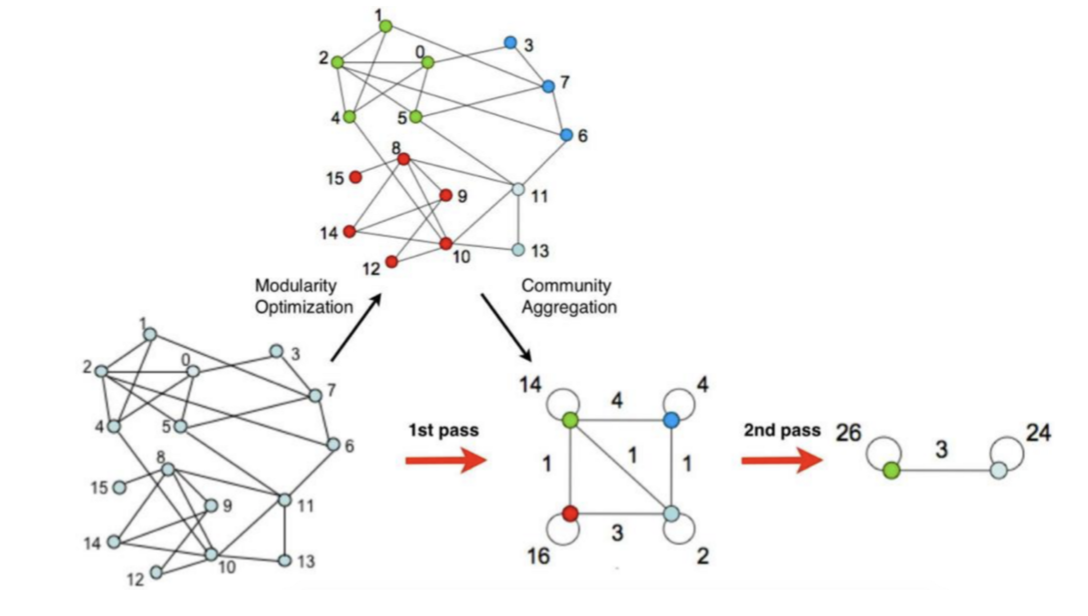
\includegraphics[width=12cm]{img/louvain.png}
  \caption{Interpretation of Louvain's Algorithm}
  \label{fig:inter}
  \end{center}
\end{figure}

\section{Experiment}

We implement Louvain's Algorithm in Python, which requires the following packages.

\begin{itemize}
    \item \texttt{networkx} a package for the creation, manipulation, and study of the structure, dynamics, and functions of complex networks.
    \item \texttt{matplotlib} for visualization of the community results
\end{itemize}

As for the graph data, we generate them from \texttt{networkx.powerlaw\_cluster\_graph}, which uses Holme and Kim algorithm for growing graphs with powerlaw degree distribution and approximate average clustering. We generate a graph with 100 nodes, with average degree of 2 and probability of adding a triangle after adding a random edge to be 0.8. We perform the Louvain's algorithm on this random graph. The running output and visualization of the community result can be found in Figure \ref{fig:code} and \ref{fig:community}.


\begin{figure}[hb]
    \begin{center}
    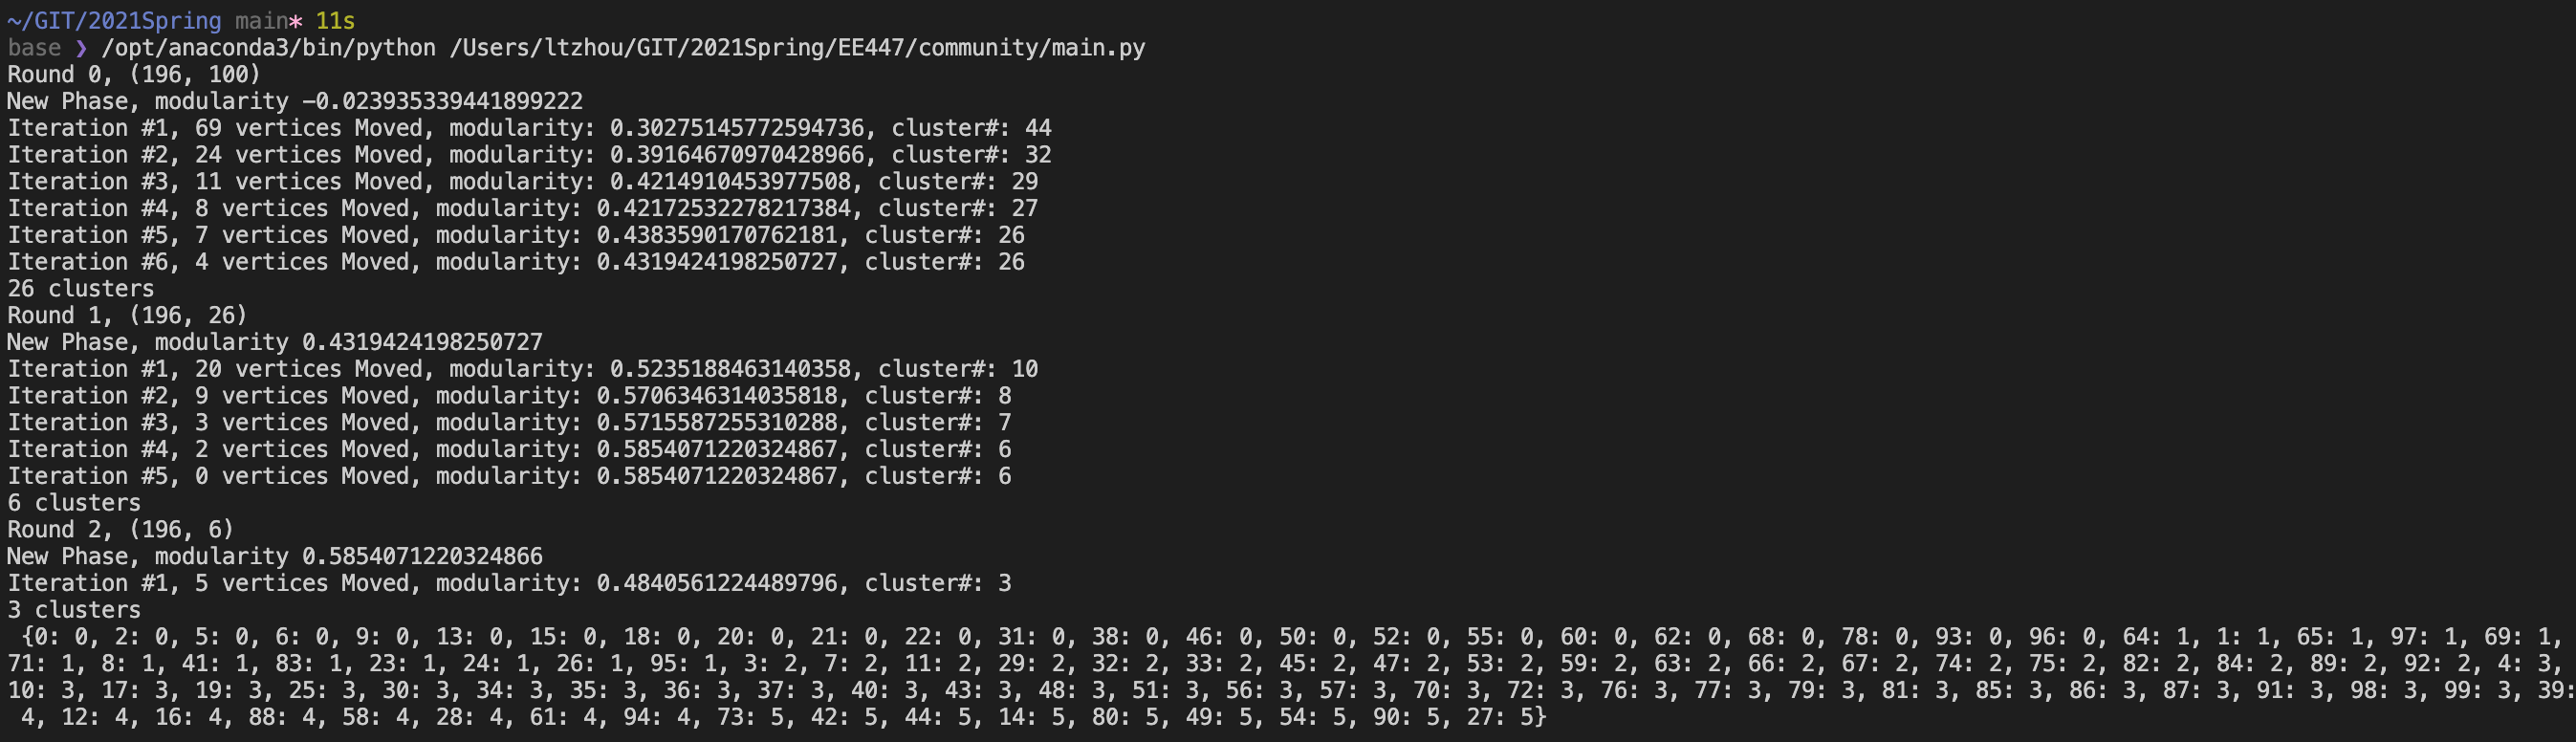
\includegraphics[width=12cm]{img/code.png}
    \caption{Execution of Louvain's Algorithm}
    \label{fig:code}
    \end{center}
  \end{figure}

\begin{figure}[hb]
  \begin{center}
  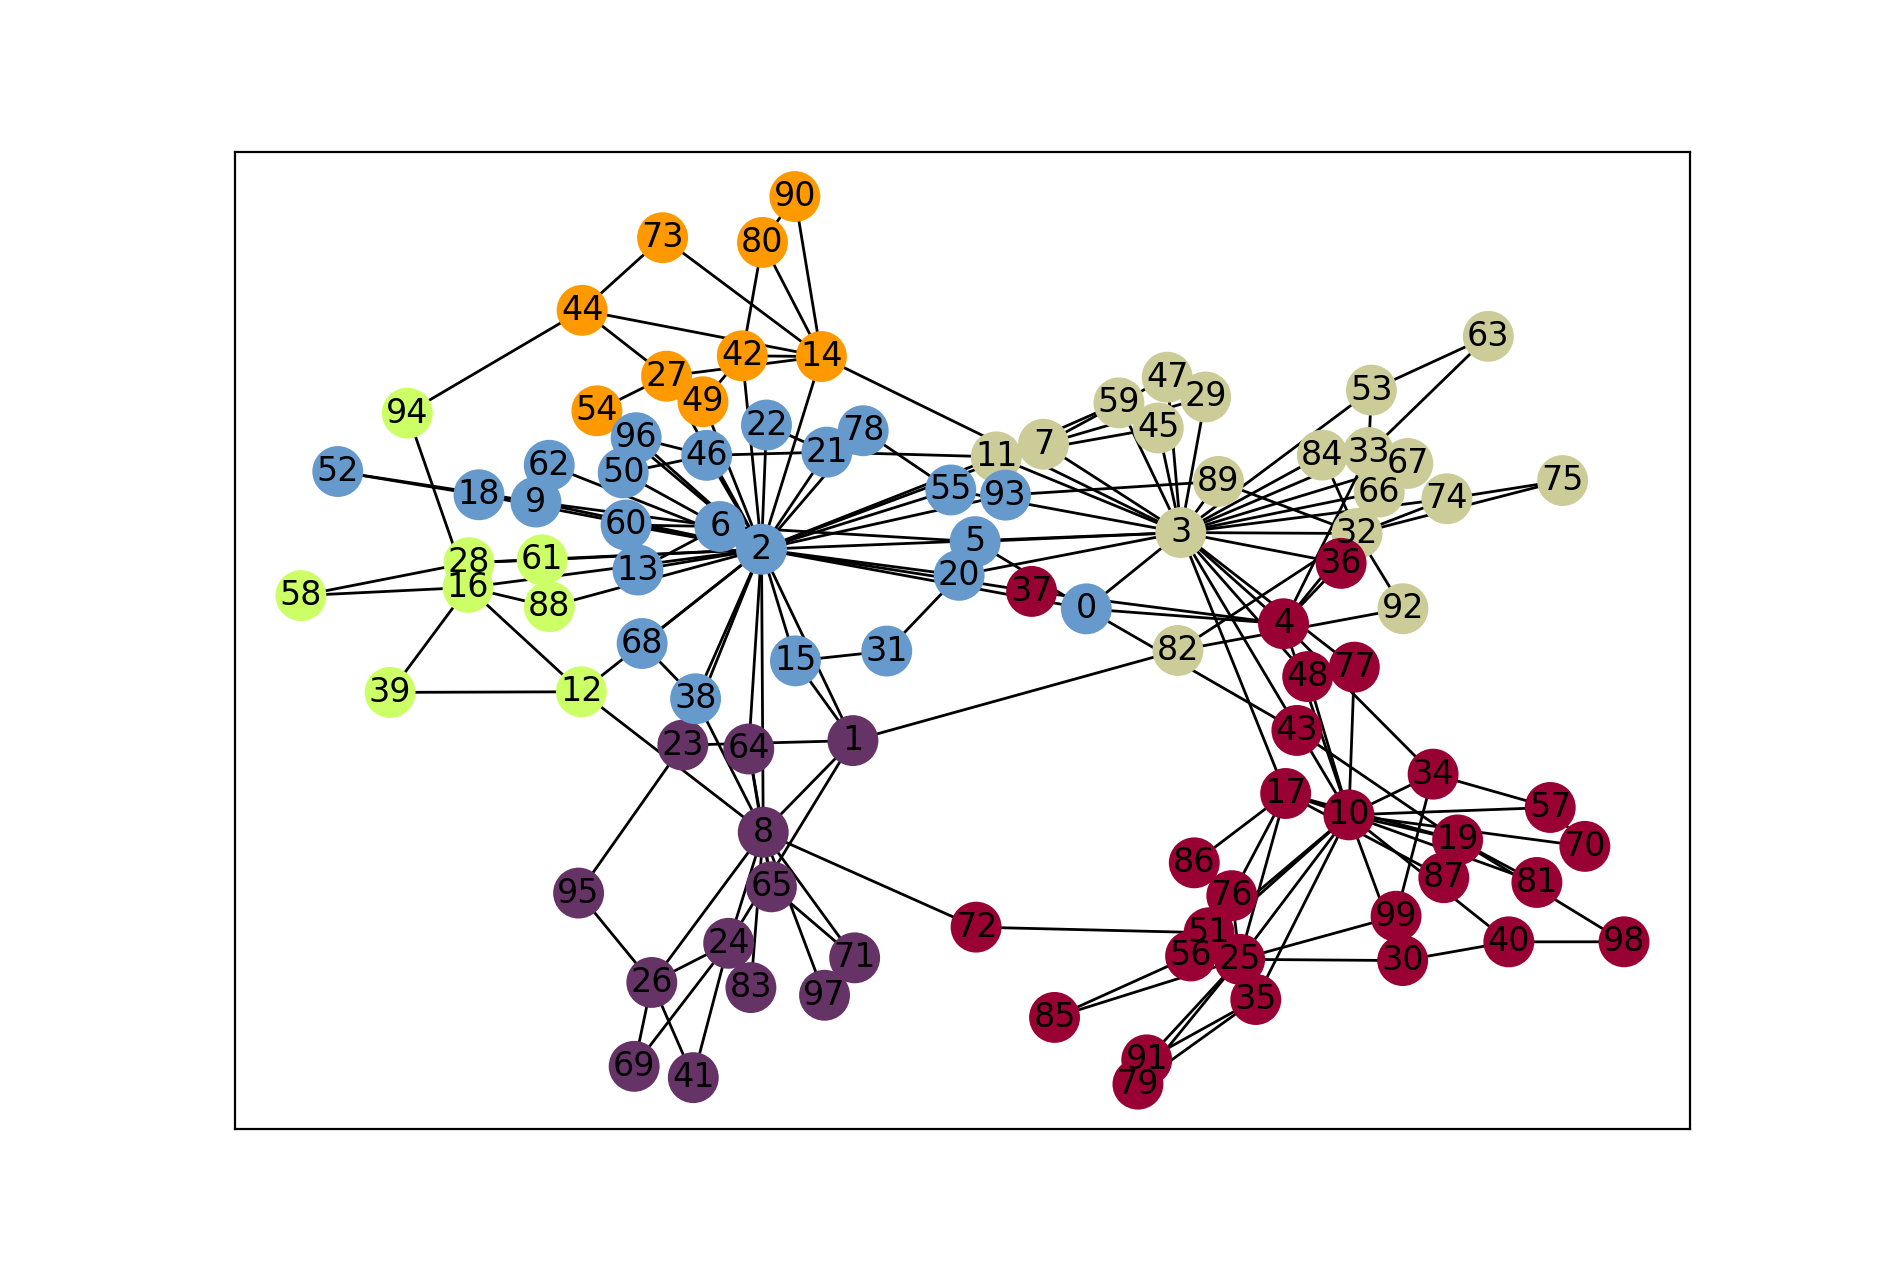
\includegraphics[width=12cm]{img/community.png}
  \caption{Visualization of Community Detection Results}
  \label{fig:community}
  \end{center}
\end{figure}

To reproduce the result, you can simply execute \texttt{python main.py}

\section{Discussions}

%%%%%%%%%%%%%%%%%%%%%%%%%%%%%%%%%%%%%%%%%%
%%%%%%%%%%%%%                 %%%%%%%%%%%%
%%%%%%%%%%%%%    EXERCISE 1   %%%%%%%%%%%%
%%%%%%%%%%%%%                 %%%%%%%%%%%%
%%%%%%%%%%%%%%%%%%%%%%%%%%%%%%%%%%%%%%%%%%
\begin{exercise}[]{Briefly describe the principle of the community detection algorithm you use.}
  \begin{solution}
  \par{~} Mentioned in Section \ref{sec:louvain}
  \end{solution}
  \label{ex1}
\end{exercise}


%%%%%%%%%%%%%%%%%%%%%%%%%%%%%%%%%%%%%%%%%%
%%%%%%%%%%%%%                 %%%%%%%%%%%%
%%%%%%%%%%%%%    EXERCISE 2   %%%%%%%%%%%%
%%%%%%%%%%%%%                 %%%%%%%%%%%%
%%%%%%%%%%%%%%%%%%%%%%%%%%%%%%%%%%%%%%%%%%
\begin{exercise}[]{In addition to visualization, what other applications does the community detection algorithm have?}
  \begin{solution}
  \par{~}
  \begin{enumerate}
      \item Reveal the correlation between nodes. Nodes that are in the same community have more similarities than those that are not. A recommendation system can be developed based on this principle.
      \item Given the community structure, we can quickly locate those links or nodes that are out of the community pattern, which may indicate a suspicious event. Some social measures can thus be built based on community detection results to evaluate the outliers.
      \item Based on community information and similarity between vertices, we can perform link prediction task for the network.
  \end{enumerate}
  \end{solution}
  \label{ex2}
\end{exercise}
